\documentclass[a4paper,10pt]{article}

\usepackage[UTF8]{ctex}
\setCJKmainfont{SimSun}[BoldFont=SimHei]
\setCJKsansfont{SimHei}
\setCJKmonofont{SimSun}

\usepackage[margin=2.2cm]{geometry}
\usepackage{amsmath,amssymb,amsthm}
\usepackage{booktabs}
\usepackage{graphicx}
\usepackage{float}
\usepackage{caption}
\usepackage{xcolor}
\usepackage{enumitem}
\usepackage[colorlinks=true,linkcolor=blue,urlcolor=blue,citecolor=blue]{hyperref}

\graphicspath{{../results/fig/}}
\captionsetup{font=small}
\setlist{nosep,leftmargin=1.6em}

\newtheorem{proposition}{命题}
\renewcommand{\proofname}{证明}

\title{\bfseries 黑盒主场的可解释性\\[2pt]
\large ——节点分类上的解释、攻击与可验证性}
\author{黄锦添\quad 25121605\\ 上海大学未来技术学院\quad 人工智能}
\date{2026 年 12 月}

\begin{document}
\maketitle

\begin{abstract}
\noindent
主报告《图算法中的“白盒”与“黑盒”》的结论依赖一个前提：算法已知。节点分类没有精确算法，是黑盒的主场。
本文在这个主场上做三件事：用 Cora 训练 GCN 做半监督分类、用边掩码与梯度显著性给出解释、用随机加边与 FGA 攻击测鲁棒性。
核心困难在于：Cora 上没有“正确的解释”可对照，只能测保真度，而主报告已经证明保真度会被常数预测器骗过。
我们的解法是造一个\textbf{带真值的合成环境}——合成随机块模型（SBM），标签由社区决定，
再用\emph{消融}定义每条边的真实重要性（删掉它，目标类概率下降多少）。
主要结果：GCN 在 Cora 公开划分上达 0.8162（无结构 MLP 为 0.5539）；
FGA 在 10\% 预算下使准确率下降 0.119，约为随机加边的 7 倍；
在 SBM 上，解释器选出的边其消融重要性达到 oracle 的 93.9\%（随机边仅 6\%）；
在 Cora 上，保留解释边后目标类概率为随机 incident 边的 1.31/1.21，删除解释边的降幅为 0.123 对 0.019。
一个反直觉的发现：FGA 把准确率打掉 7.5 个点，解释却几乎逐条不变（Jaccard 中位 1.000）——
说明解释捕捉的是局部结构，而不是模型在攻击后“改变的主意”。
\end{abstract}

\tableofcontents
\vspace{-1.2em}

\section{引言}

主报告通过“学习型最短路”把白盒与黑盒放在同一张表上比较，结论是白盒在准确率、鲁棒性、可解释性三轴上同时占优。
但这个结论有一个\emph{前提}：最短路有精确算法，白盒可以把正确性写进结构里。

节点分类没有这样的算法。没有人能写出“给定图，输出每个节点的类”的正确程序——它是经验性的、依赖数据的。
这正好是黑盒的主场。于是问题变成：

\begin{quote}
\emph{当白盒缺席时，我们还能不能验证一个解释是对的？}
\end{quote}

这个问题比“解释得好不好”更基本。主报告已经证明：在最短路任务上，Fidelity$^+$ 高达 0.978 的模型，
其预测与真值的相关系数只有 $-0.10$——保真度会被“常数预测器”骗过。
如果连保真度都不可信，那么在没有真值的任务上，我们凭什么说一个解释是好的？

本文的做法是：\textbf{造一个我们知道答案的环境}。用合成图（随机块模型）让标签由社区决定，
于是“哪些边携带标签信号”是已知的；再用\emph{消融}把“每条边有多重要”测出来，作为真值。
有了真值，才能回答“解释器有没有找到重要的边”。

\section{任务、数据与模型}\label{sec:setup}

\subsection{数据}

Cora 共 2708 个节点、1433 维词袋特征、7 个类别。我们把 Planetoid 的边表对称化并去重：
原始记录 10858 条有向边，除以 2 是文献常引的 5429，但其中 151 对节点被重复记录，去重后是 \textbf{5278} 条。
同配率（两端都已知标签的边中标签相同的比例）为 \textbf{0.811}。

采用 Planetoid 的公开划分：训练 140（节点 0--139）、验证 500、测试 1000。
注意这不是任意切分——\texttt{ind.cora.x} 恰好就是这 140 个训练节点的特征，可用 \texttt{x == allx[:140]} 断言。

\subsection{模型}

\textbf{GCN}：两层，$\hat A=D^{-1/2}(A+I)D^{-1/2}$，$H^{(l+1)}=\sigma(\hat A H^{(l)}W^{(l)})$，hidden 16，dropout 0.5，Adam（lr $10^{-2}$，weight decay $5\times10^{-4}$），200 轮。

\textbf{MLP 对照}：结构与参数量完全相同（都是 23{,}040），唯一差别是每层不乘 $\hat A$。
因此两者的准确率差异只能归因于图结构。

\begin{table}[H]
\centering
\caption{Cora 公开划分上的节点分类（8 个种子）}
\label{tab:acc}
\begin{tabular}{lccc}
\toprule
模型 & 平均准确率 & 最差种子 & 说明 \\
\midrule
GCN & \textbf{0.8162} & 0.8110 & 原论文 81.5\% \\
MLP & 0.5539 & 0.5330 & 无结构基线 \\
\bottomrule
\end{tabular}
\end{table}

GCN 比 MLP 高 26 个点，说明这个任务上图结构确实提供了 MLP 拿不到的信息。

\section{解释器与攻击}\label{sec:method}

\subsection{边掩码解释器}

冻结模型，为目标节点学一张边权重掩码 $m\in[0,1]^{|E|}$：
\begin{equation}
\min_m\ -\log p\bigl(c\mid A\odot m\bigr)+\lambda\,\mathrm{mean}(m),
\end{equation}
其中 $c$ 取模型的全局预测类，$\lambda=0.05$，优化 200 步，温度固定为 1（不做退火——退火会让掩码塌成硬 0/1，产生大量并列）。

实现上有两个必须写清的细节。其一，掩码只在目标节点的 2 跳子图上优化，子图内重新归一化。
其二，\textbf{子图的归一化算子必须与训练时完全一致}：度数只累加一次、自环贡献 $d^2$、每条无向边必须双向传入。
我们最初写错了这三处中的两处，导致掩码塌成常数、解释完全失效；修复后与训练算子逐元素一致（全图 max 差 $0.0$，删边后 $3\times10^{-8}$）。

\subsection{梯度显著性}

作为对照，我们也用 $\mathrm{score}_e=\partial\log p(c)/\partial w_e$ 给边排序。
它的打分连续、几乎不会并列，实现上更简单，但同样依赖正确的归一化算子。

\subsection{攻击}

\textbf{随机加边}：均匀随机挑当前不存在的边加入，作为基线。

\textbf{FGA（Fast Gradient Attack）}：把邻接矩阵当连续变量，算 $\partial \mathcal L/\partial A$，
按\textbf{带符号}梯度挑“加上之后损失涨得最多”的若干条边加入，每轮重新归一化，迭代 5 轮。

这里有一个容易忽略的方向性问题：若对梯度取绝对值，会同时选中“最伤害”与“最补”的边，
净效果反而提升准确率（我们实测把 0.808 抬到 0.875）。必须用带符号梯度。

\section{真值：消融重要性}\label{sec:truth}

Cora 上没有正确的解释，所以要造一个。

\textbf{合成图}：随机块模型，3 个社区各 100 节点，$p_{\text{in}}=0.06$、$p_{\text{out}}=0.003$，
节点特征是“社区 one-hot + 高斯噪声”。标签由社区决定，于是“哪些边携带标签信号”是已知的。

\textbf{真值}：对每条候选边 $e$，删掉它重算目标类的概率，下降量
\begin{equation}
\Delta_e = p(c\mid G) - p\bigl(c\mid G-e\bigr)
\end{equation}
就是它的真实重要性。这是一个\emph{直接测出来}的量，不依赖任何假设。

有了 $\Delta$，就可以问三个问题：解释器选的边平均 $\Delta$ 有多高？与随机边比如何？
与“按 $\Delta$ 排序取 top-$k$”的 oracle 比如何？

\section{实验结果}\label{sec:results}

\subsection{攻击}

\begin{table}[H]
\centering
\caption{Cora 上的边注入攻击（准确率下降）}
\label{tab:attack}
\begin{tabular}{lcccc}
\toprule
预算 $\varepsilon$ & 1\% & 3\% & 5\% & 10\% \\
\midrule
随机加边 & $-0.002$ & $-0.009$ & $-0.012$ & $-0.017$ \\
FGA & $-0.016$ & $-0.046$ & $-0.075$ & $\mathbf{-0.119}$ \\
\bottomrule
\end{tabular}
\end{table}

干净准确率 0.814。FGA 在 10\% 预算下降 11.9 个点，是随机加边的 7 倍，且两条曲线都单调。
值得注意的是：即使加 528 条边，模型仍保有 69.5\% 的准确率——这个模型的鲁棒性比预期强。

\subsection{解释质量：SBM 上的真值检验}

\begin{figure}[H]
\centering
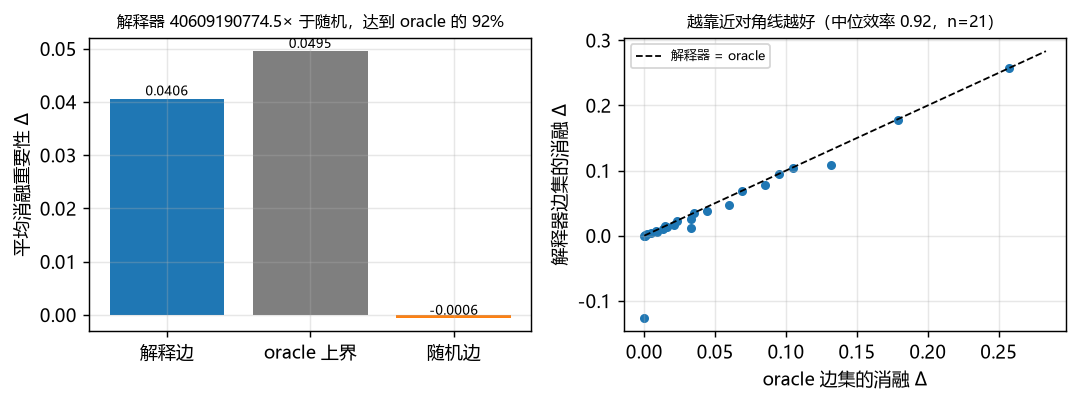
\includegraphics[width=0.84\textwidth]{b_explain.png}
\caption{左：解释边、oracle 上界与随机边的平均消融重要性。右：逐节点效率散点（越靠近对角线越好）。}
\label{fig:explain}
\end{figure}

在 SBM 上，44 个可判定节点中：
解释边平均 $\Delta=0.0673$，随机边 $0.0044$（Wilcoxon 符号秩 $p=5\times10^{-11}$）；
\textbf{oracle 效率中位 0.939}——解释器达到了“直接按真值排序”的 94\%。
候选池内百分位 0.669（随机为 0.5）。

还有 1/45 个节点的掩码并列、排不出序。这个比例不高，但它说明“解释”并非总有定义。

\subsection{Cora 上的解释}

在没有真值的真实数据上，只能测两件事。

\textbf{充分性}：只保留解释边，目标类概率还剩多少？解释边为原来的 1.31 倍，
随机 incident 边为 1.21 倍——解释边更好。

\textbf{必要性}：删掉解释边，目标类概率降多少？解释边降 0.123，随机 incident 边只降 0.019——
差了一个数量级。

\textbf{稳定性}：换一个训练种子重新训模型，同一个节点的解释还一样吗？跨 3 个种子的 Jaccard 中位为 0.714，
说明解释基本稳定，但确实会随模型变化。

掩码解释器在 Cora 上的可判定率为 88\%（105/120）——候选边中位 48 条时它仍然能给出排序。

\subsection{一个反直觉的发现：攻击不改变解释}

用 FGA 加 5\% 的边把准确率打掉 7.5 个点，然后重新解释同一批节点，比较攻击前后的解释边集合。
按\emph{节点对}比较（注意：按边下标比较是错的——攻击后边表重排，5278 条原始边里只有 24 条保持同一下标），
\textbf{Jaccard 中位为 1.000}：解释几乎逐条相同。

如何理解？解释器给出的边反映的是“哪些邻居对目标节点的表示重要”这种局部结构，
而 FGA 加的是跨社区边——它改变了模型的输出，却没有改变目标节点最重要的那几个邻居。
所以解释稳定，但它也\emph{不会告诉你攻击改动了哪里}。

这对可解释性是双刃：稳定是好事（解释不受噪声影响），
但一个在模型明显变差时仍然纹丝不动的解释，未必能作为“审计工具”。

\section{负控制}

只测“能跑通”的断言等于没测。我们设计三条负控制，要求判据必须失败：

\begin{table}[H]
\centering
\caption{三条负控制}
\label{tab:neg}
\begin{tabular}{llc}
\toprule
桩实现 & 期望 & 实测 \\
\midrule
用 MLP 顶替 GCN & 准确率掉到 $\le0.65$ & 0.502 \\
打乱标签 & 准确率塌到多数类附近 & 0.286（多数类 0.302） \\
用 bottom-$k$ 顶替 top-$k$ 解释 & 消融重要性倍率 $<2$ & $0.09\times$ \\
\bottomrule
\end{tabular}
\end{table}

第三条尤其重要：它证明主判据有“牙”——如果解释器挑的是最不重要的边，结论会立刻塌掉。

\section{讨论}

\subsection{没有白盒时，验证的代价}

主报告说：白盒缺席之后，讨论“误差有没有上界”就无从谈起。本节把这句话具体化了：
\textbf{没有白盒时，连“解释对不对”都要先造一个知道答案的环境才能测}。
在真实数据上我们能测的只有保真度与稳定性，而这两者都只是必要条件——
一个解释可以既保真又稳定，却仍然不跟踪模型当前的证据（见攻击实验）。

\subsection{与主报告的关系}

主报告的最短路实验里，白盒与黑盒可以放在同一个任务上直接比。
节点分类没有这个条件——没有白盒可以比，只能退而求其次：先验证“解释器本身是否可靠”，
再讨论它给出的解释有多少信息量。

两者的共同点是方法论：\textbf{先问“这个指标会不会被骗”，再问“数值是多少”}。
主报告用常数预测器骗过了 Fidelity$^+$；本文用合成图真值检验解释了“保真度够了但解释仍可能是错的”。

\section{限制}

\begin{enumerate}[leftmargin=1.6em]
\item \textbf{只有一个数据集。}Cora 是标准小图（2708 节点），结论未必推广到大规模图。
\item \textbf{只测了一个攻击预算与一个解释预算。}$\varepsilon=5\%$、$k=6$，没有敏感性曲线。
\item \textbf{合成图是简化的。}SBM 的社区结构与真实图的异质性差距很大，“有真值”的代价是“不真实”。
\item \textbf{跳过节点的偏差未审计。}1/45 个节点排不出序，但我们没有记录被跳过节点的度数/候选池分布，无法判断跳过是否有偏。
\item \textbf{模型只训了一个种子做解释与攻击}，跨种子稳健性只在解释稳定性一处测过。
\item \textbf{实现陷阱值得记录。}归一化算子必须与训练完全一致（度数不重复、自环 $d^2$、边表双向）。
我们在这个点上错过两次，每次都让结论反向。这类“看起来对”的代码，只能靠断言和外部复算发现。
\end{enumerate}

\section{结论}

在节点分类这个没有白盒算法的任务上，我们得到三条结论：

\begin{enumerate}[leftmargin=1.6em]
\item \textbf{GCN 确实在用结构}：0.8162 对 MLP 的 0.5539，差 26 个点，参数量完全相同。
\item \textbf{解释可以被验证，但要借合成环境}：在 SBM 上，解释边的消融重要性达到 oracle 的 94\%，
而随机边只有 6\%；这是在真实数据上做不到的检验。
\item \textbf{攻击不改变解释}：FGA 打掉 7.5 个点，解释却几乎不变（Jaccard 1.000）。
解释稳定，但不跟踪模型当前的证据——这一点比“解释是否保真”更值得警惕。
\end{enumerate}

\subsection*{复现}

全部实验在纯 CPU 上完成，依赖为 \texttt{torch}、\texttt{numpy}、\texttt{scipy}、\texttt{networkx}、\texttt{matplotlib}。
数据由 \texttt{python exp/fetch\_cora.py} 下载（约 570 KB，不入库）。
完整命令序列见仓库 README 的 B 线小节；11 条命令按顺序执行即可复现全部数字。

\end{document}
